\documentclass{article}

\usepackage[dblblindworkshop]{neurips_2026}
\workshoptitle{Africa in AI}

\usepackage[utf8]{inputenc}
\usepackage[T1]{fontenc}
\usepackage[draft]{hyperref}
\usepackage{url}
\usepackage{booktabs}
\usepackage{amsmath}
\usepackage{microtype}
\usepackage{graphicx}
\renewcommand{\topfraction}{0.9}
\renewcommand{\bottomfraction}{0.7}
\renewcommand{\textfraction}{0.07}
\renewcommand{\floatpagefraction}{0.8}
\usepackage{tikz}
\usetikzlibrary{positioning,arrows.meta,fit,backgrounds,calc}

\title{A lesson-plan-driven framework for generating\\
learning materials: a Nigerian mathematics case study}

\author{Anonymous Author(s)}

\begin{document}
\maketitle

\begin{abstract}
Preparing differentiated learning material is time-intensive for teachers, and large language
models offer a way to reduce that cost. Existing systems, however, take curriculum standards or
a seed task as the generation specification, so a generator is left to infer the lesson a class
actually received. We propose a lesson-plan-driven framework in which the artefacts a teacher
already produces are the specification: it composes curriculum objectives, the teacher's lesson
plan, subject knowledge retrieved under scope constraints, and learner state from marked class
work, and admits nothing to a learner without teacher review. We instantiate it on Nigerian
junior-secondary mathematics and compare cumulative configurations over 72 generated packs.
Four practising teachers judged the material usable --- 95 of the fully configured condition's
101 instructional-quality ratings at 4 or above --- and rated it higher on alignment with the
planned lesson than objectives-only generation, favourable ratings rising from 81.0\% to 92.2\%
and doubly rated sections with both raters favourable from 33 of 49 to 44 of 51, though six
lessons cannot take that below $p=.06$ and no component is separately established. The
learner rung adapted exactly the objectives it held evidence for and left the others
byte-identical, with raters identifying targeted error support in particular packs but no
consistent preference over the class pack. A blinded judge, reported separately, orders the
configurations the same way. The contribution is an implemented framework that makes
teacher-authored instructional knowledge explicit in educational generation, with a locally
situated evaluation of both its rungs.
\end{abstract}

\section{Introduction}

Producing the material a lesson requires --- explanation, worked examples, practice and
assessment --- is a substantial, recurring part of a teacher's workload
\citep{ajayi2015,instructionalagents2025}, and it is typically authored once for a whole class.
Differentiated instruction asks for more: that content, process and product vary with learners'
readiness, interest and pace \citep{tomlinson1999}, an expectation personalised-learning
research has since made explicit \citep{bernacki2021}. That expectation is additive: it does not
replace existing preparation but multiplies it by class size, and must be met inside curricula
prescribing what is covered and when \citep{nikolaidis2024}; teachers accordingly want AI to
complement rather than replace their judgement \citep{seo2024}.

Large language models can supply part of that capacity, generating explanations
\citep{leinonen2023}, worked examples \citep{jury2024} and controllable practice questions
\citep{li2024}, with \citet{sharma2025} surveying the effect on personalised learning. What is
missing is an account running from planning to delivery. Existing systems take curriculum standards or a seed task as the generation
specification \citep{cogent,facet,lectura}, so a generator must infer how the topic was
approached, in what order, and against which anticipated errors; the material reflects the
curriculum rather than the lesson a class received. Nor is it settled how
learner evidence should enter such a pipeline \citep{cho2024}.

Teachers already produce the missing specification. Planning is routine, documented practice
\citep{yinger1980,musingafi2015}: a lesson plan precedes each lesson, a lesson note derives from
it, and marked class work accumulates as teaching proceeds. We ask whether these artefacts can
drive generation of downstream material, and whether the marked work can then personalise it,
without additional authoring. We address this through design science research
\citep{hevner2004,peffers2007}, in which the contribution is a designed artefact whose
objectives are inferred from the problem. The artefact is a lesson-plan-driven framework,
adapting the component decomposition of classical intelligent tutoring systems
\citep{wenger1987,nwana1990}: it separates curriculum objectives, a lesson-plan specification,
scope-constrained subject knowledge, and learner state from marked class work, and admits
nothing to a learner without teacher review.

Two design objectives follow, which \citet{hevner2004} require be demonstrated rather than
asserted, so we restate them as testable claims. \textbf{H1}: material generated under a
lesson-plan specification aligns better with the taught lesson and its curriculum objectives
than material generated from curriculum objectives alone. \textbf{H2}: material generated under
a learner state derived from marked class work addresses an individual pupil's learning better
than generic class-level material. We evaluate both. Our contributions are:

\begin{itemize}\itemsep2pt
\item \textbf{A formal lesson-plan-driven generation framework.} We represent teacher-authored
lesson plans as explicit instructional specifications and integrate them with curriculum
objectives, subject knowledge, target-material requirements and objective-level learner state in
an ITS-inspired generation-and-validation framework under teacher review.
\item \textbf{A situated evaluation of usefulness and teacher alignment.} We instantiate the
framework in Nigerian JSS1 mathematics and compare cumulative configurations across 72 generated
packs, giving evidence of educator-assessed usefulness and higher observed teacher-planned
lesson alignment in the fuller configurations than in objectives-only generation.
\item \textbf{A demonstration and evaluation of selective personalisation.} We evaluate
learner-specific adaptation across 26 learner-lesson cases, verify preservation of sections
outside the recorded adaptation scope, and document educator-identified examples of targeted
error support, distinguished from the stronger claim of a consistent advantage over class-level
material.
\end{itemize}

\section{Related work}

Two lines of work are relevant. The first generates learner-facing material from a curriculum
specification. \citet{cogent} propose COGENT, producing grade-appropriate passages from NGSS
concepts; \citet{facet} present FACET, generating a differentiated worksheet from a seed problem
with a learner simulated from two binary traits; \citet{lectura} describe Lect\=uraAgents, which
assembles lecture packages from a syllabus it writes itself. LearnLens couples error-aware
assessment with curriculum-grounded generation under educator oversight \citep{zhao2025} and
GenMentor schedules a learning path from a learner's goal \citep{wang2025};
\citet{holstein2020} frame the division of adaptive work between teacher and system.

The second line generates \emph{lesson plans}: \citet{ranawat2021} sequence web-annotated
plans, \citet{moundridou2024} implement inquiry-based ones, \citet{olaniyan2025} align generated
plans to Bloom's taxonomy, \citet{zhang2025} and \citet{zheng2025} propose multi-agent and
knowledge-grounded plan generation, and \citet{celik2026} study pre-service teachers
co-constructing plans with a model. Closest to our setting, \citet{dennison2026} report Shiksha
Copilot, with which teachers in low-resource schools curate and customise generated plans. Our
position is the converse: these systems treat the lesson plan as an \emph{output}, whereas we
treat an existing teacher-authored plan as the \emph{input} constraining generation of other
material. We are aware of no prior system that takes the plan in that role.

Two further gaps are methodological. These systems introduce several capabilities together and
evaluate the assembled pipeline against a baseline, so the field has end-to-end results without
evidence about which components produce them; we are aware of no published component-additive
ablation of an educational LLM generation system. And the three closest comparators evaluate with
expert human raters, yet none reports an inter-rater reliability statistic or validates its judge against its
humans, and Lect\=uraAgents assigns one rater per item, so reliability there is uncomputable.
We measure ours in \S\ref{sec:human}.

\section{The framework}
\label{sec:framework}

Teachers already record what they intend to teach and what their pupils did with it. The
framework takes those records as the specification a generator works from: the plan says what
the lesson was, the note carries its subject matter, marked class work the evidence about each
pupil. The generator, the source retrieval reads and the kind of material produced are left
open.

Five design principles fix what any implementation must satisfy. The lesson plan is the binding
specification, constraining content to its scope and objectives (\textbf{DP1}), since curriculum
standards alone leave the generator to infer the lesson. Teacher
approval precedes learner access, as a non-optional gate with an audit record (\textbf{DP2}),
and personalisation is constrained so that difficulty may vary but topic scope may not
(\textbf{DP4}): teachers ask that AI complement their judgement \citep{seo2024} inside a
curriculum prescribing what is covered and when \citep{nikolaidis2024}. Every item carries an
objective tag and a provenance link (\textbf{DP3}), so material can be checked against the lesson it
serves. And generation happens ahead of time, separating model-dependent
preparation from learner use (\textbf{DP5}), for a school that cannot depend on a model at the
point of use; this last we do not evaluate. Only DP1 and DP2 are structural: an instantiation without the lesson plan or the review gate is
not an instance of this framework, while retrieval, validation and the learner state may be
present or absent.

Four layers realise those principles (Figure~\ref{fig:framework}). The \textbf{specification}
layer holds the objects generation is conditioned on. In the classical decomposition
\citep{wenger1987,nwana1990} a domain model represents the subject matter and what counts as
correct performance; here retrieval supplies the former and the curriculum the latter. Learner
state is the student model, and the lesson plan stands in for a tutoring model the system would
otherwise infer. The layer also imposes four
curriculum constraints on the output: \emph{scope} (only units in the current period), \emph{coverage} (every objective
addressed), \emph{resource} (only mapped sources) and \emph{sequence} (prerequisites from
earlier periods). The \textbf{generation} layer projects those objects into a request, drafts and
validates it; the \textbf{governance} layer decides what reaches a learner; and
\textbf{delivery} sits outside the generation path.

\begin{figure}[!tb]
\centering
\newcommand{\dsc}[1]{\\[-3pt]{\scriptsize #1}}
\newcommand{\its}[1]{\\[-2pt]{\scriptsize\itshape\textcolor{black!55}{#1}}}
\scalebox{0.78}{
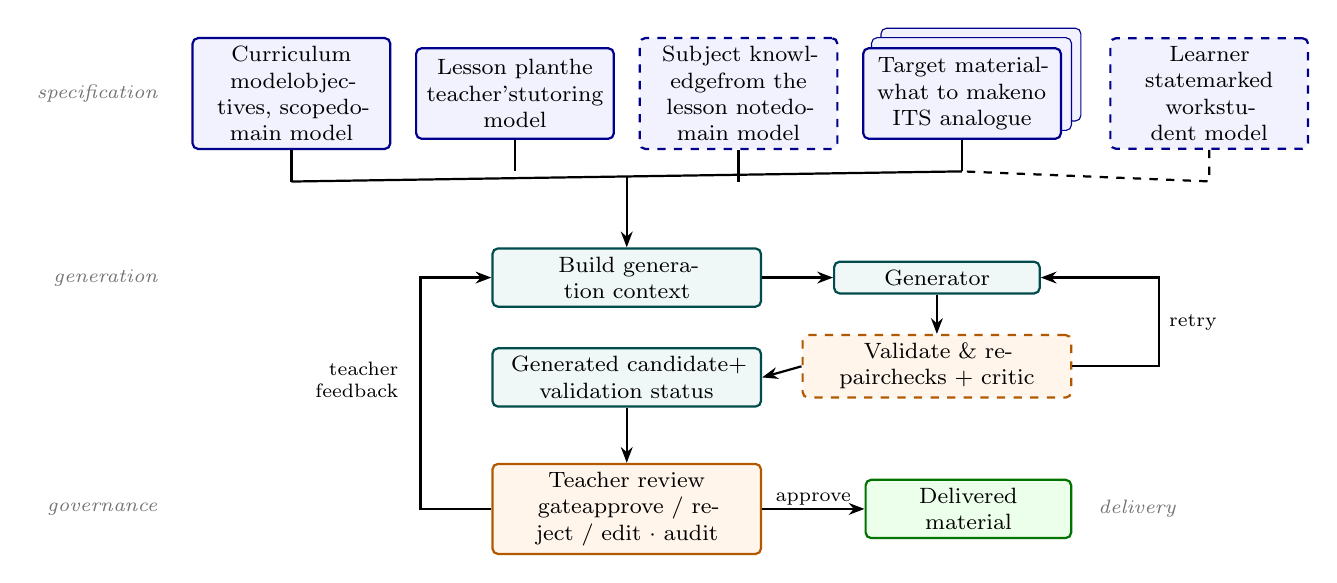
\begin{tikzpicture}[
  font=\small,
  box/.style={draw,rounded corners=2pt,align=center,inner sep=3pt,fill=white,
              font=\footnotesize},
  sbox/.style={box,draw=blue!55!black,fill=blue!5,minimum height=11.5mm},
  gbox/.style={box,draw=teal!60!black,fill=teal!6},
  vbox/.style={box,draw=orange!70!black,fill=orange!8},
  dbox/.style={box,draw=green!45!black,fill=green!8},
  lay/.style={font=\scriptsize\itshape,text=black!55},
  tag/.style={font=\scriptsize,inner sep=1pt,text=black!70},
  ->,>={Stealth[length=2mm]},thick
]
\node[sbox,text width=23mm] (cm)
  {Curriculum model\dsc{objectives, scope}\its{domain model}};
\node[sbox,text width=23mm,right=3mm of cm] (lpr)
  {Lesson plan\dsc{the teacher's}\its{tutoring model}};
\node[sbox,text width=23mm,right=3mm of lpr,dashed] (exp)
  {Subject knowledge\dsc{from the lesson note}\its{domain model}};
\node[sbox,text width=23mm,right=3mm of exp] (spec)
  {Target material\dsc{what to make}\its{no ITS analogue}};
\node[sbox,text width=23mm,right=6mm of spec,dashed] (ls)
  {Learner state\dsc{marked work}\its{student model}};
\coordinate (busL) at ($(cm.south)+(0,-4mm)$);
\coordinate (busR) at ($(spec.south)+(0,-4mm)$);
\coordinate (busM) at ($(busL)!0.5!(busR)$);
\foreach \n in {cm,lpr,exp,spec} \draw[-] (\n.south) -- ($(\n.south)+(0,-4mm)$);
\draw[-] (busL) -- (busR);
\draw[dashed,-] (ls.south) -- ($(ls.south)+(0,-4mm)$) -- (busR);

\node[gbox,text width=32mm,below=9mm of busM] (ctx) {Build generation context};
\node[gbox,right=9mm of ctx,text width=24mm] (gen) {Generator};
\node[vbox,below=5mm of gen,text width=32mm,dashed] (val)
  {Validate \& repair\dsc{checks $+$ critic}};
\node[gbox,below=5mm of ctx,text width=32mm] (cand)
  {Generated candidate\dsc{$+$ validation status}};
\node[vbox,below=7mm of cand,text width=32mm] (trg)
  {Teacher review gate\dsc{approve / reject / edit $\cdot$ audit}};
\node[dbox,right=13mm of trg,text width=24mm] (del) {Delivered material};

\draw (busM) -- (ctx.north);
\draw (ctx) -- (gen);
\draw (gen) -- (val);
\draw (val.east) -- ++(11mm,0) |- node[pos=0.25,right,font=\scriptsize] {retry} (gen.east);
\draw (val.west) -- (cand.east);
\draw (cand) -- (trg);
\draw (trg) -- node[font=\scriptsize,above,inner sep=1pt] {approve} (del);
\draw (trg.west) -- ++(-9mm,0) |- (ctx.west);
\node[font=\scriptsize,align=right,anchor=east] at ($(ctx.west)+(-10.5mm,-13mm)$)
  {teacher\\feedback};

\begin{scope}[on background layer]
\foreach \d in {2.4,1.2}
  \draw[rounded corners=2pt,draw=blue!55!black,fill=blue!5]
    ($(spec.south west)+(\d mm,\d mm)$) rectangle ($(spec.north east)+(\d mm,\d mm)$);
\end{scope}

\coordinate (lx) at ($(cm.west)+(-3mm,0)$);
\node[lay,anchor=east] at (lx) {specification};
\node[lay,anchor=east] at (lx|-ctx) {generation};
\node[lay,anchor=east] at (lx|-trg) {governance};
\node[lay,right=2mm of del] {delivery};

\end{tikzpicture}}
\caption{The framework. The tutoring components it adapts are named in italic, and dashed
boxes are optional: an instance may omit retrieval, validation or the learner state. The target
material is drawn as a stack because substituting it changes what is produced --- a lesson
note, a worksheet, an assessment --- without changing the components that supply it. The target
material and the review gate have no counterpart in that decomposition --- they are what
generating content, rather than selecting it, requires. The gate is a decision point: an
approved pack is delivered, and teacher feedback returns the material to generation.}
\label{fig:framework}
\end{figure}

\subsection{The specification layer}
\label{sec:plan}

Systems that generate educational content typically condition on curriculum objectives. Let a
curriculum unit carry an ordered set of objectives $O=(o_1,\dots,o_n)$, each a sentence of the
form \emph{carry out order of operation in algebra}. An objective specifies what a learner
should be able to do at the end of a unit, but not how instruction reached that outcome.

A lesson plan specifies the latter. Written before the lesson and structured by the national
format, it records a teacher's decisions about one session. \citet{yinger1980} describes
planning as a staged process in which a teacher formulates and resolves an instructional
problem before delivery, and \citet{biggs1996} argues that alignment between objectives,
activities and assessment is what makes such planning instructionally effective. The plan is
where both are recorded. We represent it as
\begin{equation}
P \;=\; \langle\, O_P,\; S,\; A,\; E,\; K,\; M \,\rangle ,
\label{eq:plan}
\end{equation}
where $O_P$ are the lesson objectives the teacher derived from $O$, $S$ an ordered sequence of
instructional steps, $A$ the assessment she planned, $E$ the entry behaviour she assumes, $K$
the misconceptions she anticipates and $M$ her materials. Each step is
$s=\langle\rho,\kappa,o,T\rangle$: a structural role $\rho\in\{\textsc{intro},\textsc{core},
\textsc{eval}\}$, the kind of knowledge $\kappa\in\{\textsc{concept},\textsc{procedure},
\textsc{representation}\}$ a core step teaches, the objective $o\in O_P$ it serves, and the
activities $T$ it sets. $P$ therefore differs from
$O$ in kind rather than in detail: a sequenced, typed record of the instruction planned to reach
the outcomes $O$ names.

Two further objects complete the layer. The target material is a first-class input, so the
framework is not tied to one output type; adaptation additionally requires learner evidence, for
which we use the marked class work a school already holds. For pupil $\ell$ and objective $o$,
\begin{equation}
\Sigma = \langle\, \alpha,\; \beta,\; R \,\rangle ,
\qquad
\Lambda(\ell,o) = \langle\, b,\; m,\; c,\; d,\; \mu,\; V \,\rangle ,
\quad b \in \{\textsc{remediate},\textsc{reinforce},\textsc{extend}\} .
\label{eq:spec}
\end{equation}
$\Sigma$ names the material kind $\alpha$, its audience $\beta$ and the requirements $R$ it must
satisfy; substituting it changes what is produced --- a lesson note, a revision worksheet, an
assessment --- without changing the components that supply it. In $\Lambda$, $b$ is a mastery
band, $m$ the evidence supporting it (a count over items, not a bare fraction), $c$ and $d$ the
pupil's confidence and perceived difficulty, $\mu$ any diagnosed misconception and $V$ the marked
answers. $\Lambda$ is indexed by objective, not by pupil: a learner may need extension on one
objective and remediation on the next.

\subsection{The generation layer}
\label{sec:repr}

A plan is not supplied to the model in full. A policy $\theta$ projects it onto the input for a
single output section,
\begin{equation}
\pi_\theta : (P,o) \;\longmapsto\; U ,
\label{eq:proj}
\end{equation}
declaring field by field what travels. In our instantiation $\theta$ codes the teacher's
narration as instructional events and drops the raw prose, carries lesson-level materials on the
lesson context rather than per step, and withholds step titles because most restate the
objective. Generation is then $G(\Sigma,U)\mapsto Y$, producing a section $Y$ against the
objective it addresses, and $\mathcal{V}$ validates the draft against the constraint schema.

Two operators complete the layer. Scoped retrieval $\varrho(o)$ adds evidence for the
objective, and a validation-and-repair operator $\mathcal{V}$ checks the draft against the
constraint schema and repairs what fails. Because $\theta$ is declared rather than implicit, an
instance's inputs can be varied one at a time --- which is what makes the design evaluable
component by component.

\subsection{The governance layer}

Nothing reaches a learner without teacher approval, and the gate is a decision rather than a
formality: a pack is approved, rejected, or returned to generation with the teacher's feedback,
and the decision is recorded with its reason (\textbf{DP2}). A returned pack re-enters as a
revision turn constrained to the same objective set, so review can change what a section says
but cannot quietly drop an objective the plan requires. Delivery is separate again: packs are
compiled ahead of use (\textbf{DP5}), so the model is needed when a teacher prepares, not when
a pupil reads.

\subsection{Binding and cost}

The framework's terms bind to a local curriculum vocabulary: in the Nigerian NERDC curriculum a
unit is a subtopic and objectives are performance objectives, the basis of the claimed
reusability and an argument from structure, since we evaluate one binding here. Constraints are
\emph{supplied} and the output \emph{checked} against them --- a mechanism, not a guarantee,
since schema validity establishes neither mathematical correctness nor faithful sequencing ---
and teacher approval is a governance component, distinct from $\mathcal{V}$.

Manual differentiation scales with teacher time per pupil; here a second pupil's pack costs one
further generation call over the same specification plus $\Lambda(\ell,o)$, from work already
marked, with no new authoring and no live model at the point of use. Teacher effort shifts from
authoring to review --- a property of the design, not a measured saving.

\section{Instantiation}
\label{sec:instantiation}

We demonstrate the framework on Nigerian junior secondary mathematics (JSS1, pupils aged
roughly 11--13) in a class of forty taught by one teacher, a setting with limited capacity for
manual differentiation. \citet{musingafi2015} describe how curriculum expectations pass through
syllabi and schemes of work into the lesson plan, where a teacher fixes objectives, sequence and
assessment for one session; in Nigerian schools \citet{ajayi2015} report uneven competence in
preparing such lessons and \citet{ayovaughan2022} variation in whether the prescribed formats
are used, so a framework consuming plans must accept what teachers actually write. The study uses
the materials the school produces for every lesson, a lesson plan and a lesson note, which the
framework consumes directly.

The framework produces the material named by $\Sigma$. Here $\Sigma$ specifies a post-class
revision pack, a self-study document a pupil works through at home, and holds the output
requirements fixed across conditions: its kind $\alpha$ is ``one section of a take-home revision
pack'', its audience $\beta$ a JSS1 pupil revising alone at home, and its five requirements $R$
fix the register (never about the lesson as an event), the title, the topic scope, the presence
of answers, and what a section may refer to. Substituting a different $\Sigma$ --- an exit
ticket, a worksheet --- changes the material without changing the components that supply it.

Each unit $U$ is keyed to one objective, so a pack has one section per objective. Within
$\pi_\theta$ the narration in $T$ is coded as Gagn\'e instructional events \citep{gagne1985} by
a deterministic rule set: one code per activity, weak evidence uncoded, duplicates collapsed.
Five of the nine events occur here and the other four are never inferred, so the coding
describes the lesson the teacher planned, not one the framework recommends. For lesson t2-w09 and $o=$ \emph{carry out order of operation in algebra},
$\pi_\theta(P,o)$ carries the step's position in $S$, the events \textsc{guidance},
\textsc{performance} and \textsc{feedback}, the four items she set ($4n+3n\times10$,
$32+8x\div2$, $3\times5x+4x\div2$, $36y\div6+y+2\times4y$) and her assessment; under C0 the
unit is $U_0=\langle o\rangle$ and carries none of it. The C1 pack practises on her items, the
C0 pack on three it generates itself ($3x+2\times4x$, $5(2x+3)$, $4x+3(2x-1)$) without the
division hers exercise. Reuse of her exercises is not the criterion: newly generated
exercises may equally satisfy $\Sigma$, and fidelity concerns the instructional requirements
rather than reuse.




\section{Evaluation design}
\label{sec:design}

The class-level ablation was evaluated on two independent instruments applied to the same 72
packs: a blinded LLM judge and a panel of practising teachers. We report both, rather than
the one that separates.

\paragraph{Corpus.}
Six lessons were drawn from two terms of the teacher's own record, covering 17 learning
objectives, and each of the four class-level settings generated three independent draws per
lesson, giving $6\times4\times3=72$ packs. The corpus additionally holds the marked class work
of nine pupils across three lessons, sampled by stratified random selection over the teacher's
ability categories, which were not themselves recorded, so we report no stratum result. The
stratum determines whom we sample; $\Lambda$ responds to objective-level evidence.

\paragraph{Conditions.}
Each condition is a setting of the projection policy $\theta$ over one architecture, adding a
component at a time (Table~\ref{tab:conditions}). Because $\Sigma$, the generator and the
output contract are fixed, a rung's effect is that component's effect.

\begin{table}[!htbp]
\centering
\small
\caption{The ablation. Inputs are cumulative. C0 supplies the objective alone --- the
framework with its specification removed, and so not an instance of it. Retrieval is capped at
three evidence items per unit with source references required; $\mathcal{V}$ runs eight
structural checks and an LLM critic with up to two repair retries.}
\label{tab:conditions}
\begin{tabular}{llll}
\toprule
& Unit supplied to $G$ & Component added & Evaluated here \\
\midrule
C0 & $U_0=\langle o\rangle$ & Objective only & yes \\
C1 & $\pi_\theta(P,o)$ & The teacher's lesson plan & yes \\
C2 & $\pi_\theta(P,o)\cup\varrho(o)$ & Scoped retrieval over the lesson note & yes \\
C3 & C2's unit, then $\mathcal{V}$ & Validation and repair & yes \\
P1 & C3's unit $+\;\Lambda(\ell,o)$ & Learner state from marked work & yes \\
\bottomrule
\end{tabular}
\end{table}

\paragraph{Criteria.}
The human panel scores three constructs: whether the material addresses the stated objective
(\emph{curriculum-objective alignment}); whether it reflects the lesson as planned
(\emph{lesson-specification fidelity}, the primary construct, which operationalises H1); and
whether it is mathematically correct, clear and useful (\emph{instructional quality}), each
1--5 against fixed descriptors. The judge scores four dimensions on the
same scale, quality split into correctness and clarity; we report the primary construct alone
as well as the composite.

\paragraph{Primary comparison.}
The comparison of primary interest is the lesson-plan-bearing family (C1--C3) against the
objectives-only baseline (C0), with diagnostics C1$-$C0, C2$-$C1 and C3$-$C2 locating any
effect. The endpoint frozen
before data collection --- internally recorded, not publicly registered --- was C1 versus C0 on
the human panel; the family contrast was adopted afterwards, once judge scores had been
inspected, and is exploratory, as are the diagnostics, whose $p$-values are unadjusted.

\paragraph{The judge.}
The LLM judge (Claude Sonnet 4.6) is blinded to condition and is constrained in code to
differ from the generator. It was run twice over all 72 packs in fully independent passes, so its
repeat reliability could be measured before its scores were interpreted.

\paragraph{The human panel.}
Four practising mathematics teachers rated packs on the three criteria per objective, blind to
condition and with delivery order counterbalanced. We report their scores as levels, as
condition means and favourable rates, and as what the two raters of a section agreed on, rather
than through a model that would have to assume how rater variance enters.

\paragraph{Implementation and aggregation.}
All 72 packs were generated by DeepSeek-V4-Flash at temperature 0 with caching disabled, using a DSPy 3.3.0 harness \citep{dspy}: our own
composition module driving a ReAct-style tool loop \citep{react}, evidence
in-prompt, rewrite-style repair. DSPy is a programming framework here; no prompt-optimisation
procedure was run. The same model and harness generated every condition. Per lesson and
condition,
judge scores average over three packs and both passes; C1--C3 are weighted equally within a
lesson, compared with C0, and the six lesson differences averaged equally.

\section{Results}
\label{sec:results}

\subsection{The components executed}

Before asking whether the rungs differ in quality we verify from the generation log that they
differ at all, with no rater involved. Retrieval attaches source references to 168 blocks at C2
and 157 at C3, around 58\%, and none at C0 or C1 where it is disabled; the validator ran on all
18 C3 packs and no others, logging 76 findings, a mean of 4.22 per pack.




\subsection{What the human panel could resolve}
\label{sec:human}

The panel returned 1{,}212 of 1{,}224 planned scores, with delivery position balanced across
conditions by design (ANOVA, $F=0.01$, $p=.998$). Read as levels rather than differences, the material is judged usable: on instructional quality
95 of C3's 101 ratings are at 4 or above and both raters were favourable on 44 of its 50 doubly
rated sections. C0 is high there too, at 93 of 100, so the panel does not separate the
conditions on quality.

It separates them on the criterion H1 names (Figure~\ref{fig:alignment}). Across C0--C3 the
lesson-context means run 4.26, 4.34, 4.53 and 4.58, and sections where either rater went to 2 or
below fall 5, 2, 1, 0.

\begin{figure}[!tb]
\centering
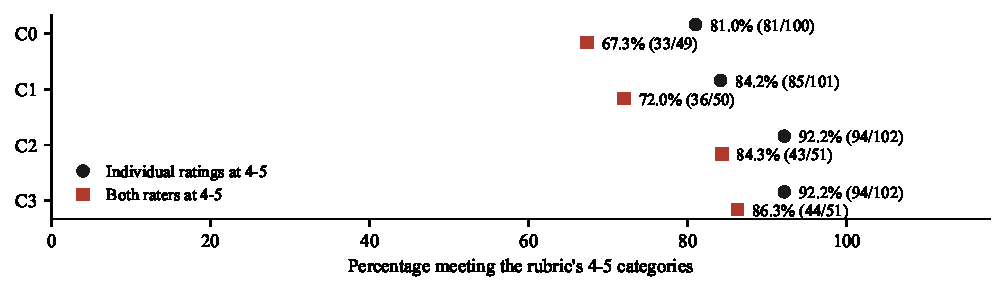
\includegraphics[width=0.84\textwidth]{alignment.pdf}
\caption{Teacher-planned lesson alignment, as individual favourable ratings and as sections
both raters marked favourably. Denominators differ because 12 assigned ratings were not
returned.}
\label{fig:alignment}
\end{figure}

One difference per lesson puts C3 ahead of C0 in five of six lessons and level in the sixth, by
$+0.283$; C2 by $+0.190$ (4/6), C1 by $+0.068$ (3/6), the equally weighted family by $+0.180$
(4/6). Six lessons put the exact signed-rank floor at $p=.0625$, where C3 lands: consistent
across lessons, no single rung separately established.

Curriculum-objective alignment sits at 90--94\% at 4--5 in every condition, which is why we
read the focal criterion rather than the three-criterion composite --- a decision taken after
the protocol, which named the composite.

What limits the reading is the raters, not the material. On this criterion their means run
4.57, 4.47, 4.56 and 4.12 and their favourable rates 88.7\%, 96.0\%, 86.5\% and 78.8\%, and the
two raters of a section differ by two points or more on 10 of C0's 49 sections, 9 of 50, 6 of 51
and 5 of 51. Disagreement falls as the configuration fills, but never to a level at which the
panel could resolve a rung on its own.

It is a stable instrument: run twice in fully independent passes over the same 72 packs it moved
a score by 0.076 on average and returned an identical score on 92.4\% of 288 comparisons, with no
justification string byte-identical between passes.


\subsection{What the automated judge adds}


On the judge the lesson-plan-bearing family scores above the objectives-only baseline in every
one of the six lessons, exceeding C0 on the primary construct by $+0.750$ (Wilcoxon signed-rank,
two-sided $p=.031$).

The diagnostics locate most of that difference at one rung: adding the lesson plan moves the
primary construct $+0.694$ (5/6, $p=.0625$), retrieval a further $+0.111$ (3/6) and validation
$-0.056$ (0/6). That is evidence the plan carries most of the family effect and no evidence of
further contribution, not evidence the contribution is zero.



\paragraph{The difference is concentrated in low-score flags.}
Of the 18 objectives-only packs, 8 carry at least one judged
score below 4; of the 54 generated with a lesson plan, none does (Fisher exact
$p = 3.7 \times 10^{-6}$), an operationally defined flag rather than a confirmed defect.

They are construct-specific: 8 of 18 C0 packs on lesson-specification fidelity, against 1 on
curriculum-objective alignment, 1 on conceptual correctness and none on clarity.

\paragraph{The validation component did not close.}
The validator closed its repair loop on only 6 of the 18 C3 packs; the other 12 exhausted both
retries still carrying a finding, consistent with that rung showing no gain.

\subsection{The learner-model rung}
\label{sec:h2}

Part 2 put each pupil's personalised pack against the class base pack: 26 learner-lesson cases
over nine pupils and three lessons, 35 objective panels rated by two teachers each on opposite
orders, 199 of 210 cells answered.

Personalisation was selective, a property of the generation record rather than a judgement:
compared section by section within an objective, P1 changed exactly the 35
objectives for which it held learner state and left the 34 it did not byte-identical.

The comparative judgement goes no further. Scoring each judgement $+1$ for P1, $0$ for about the
same and $-1$ for P0, and weighting pupils equally, P1 exceeds P0 by $+0.045$ (stratified
cluster bootstrap over the nine pupils, $[-0.106,+0.199]$); the direction varies by criterion: P1 on 38 of 67 adaptive-calibration judgements, 25 of 67 for learner-evidence alignment against 24, and 20 of
65 for instructional integrity against 25. On adaptive calibration the two raters chose
opposite materials on 11 of 32 doubly rated panels. Comments were optional; 15 cells carry one, and
some identify targeted support --- one records that the personalised section ``repeatedly laid
emphasis on the mistake and carefully broke the steps down''. Instances, not a rate.

\section{Discussion}

Teachers judged the material usable and rated the fuller configurations higher on alignment
with the lesson they had planned; the automated judge orders the configurations the same way.
Neither instrument establishes a separate contribution for any one component --- the increase
concentrates where the plan enters, and retrieval adds no measured gain, though it attaches
source references to roughly 58\% of blocks, a traceability aggregate ratings were not designed
to detect. On H2 the mechanism and the judgement come apart: personalisation was exactly as
selective as the design intends, and teachers still did not prefer its output. Adoption also
depends on teacher readiness, which \citet{ayanwale2025} model for the Nigerian context.

\section{Limitations}

Five limitations bound these results. First, both instruments have known limits: the judge is
validated for repeat stability but not against human judgement, and the panel's pooled agreement is
weak, so neither result rests on a reference we can call reliable.
Second, C0 is our own pipeline with its inputs removed, so the ablation establishes internal
attribution, not external superiority. Third, the evidence does not travel far from the case
that produced it --- one subject, one grade, one school, six lessons, one generator --- so the
framework's reuse remains an argument from structure. Fourth, we evaluate material and not
learning: there is no pre-test, post-test or retention measure, and H2's instrument asks which
of two documents a teacher prefers, not whether either taught anything.
Finally, we did not measure the workflow burden that motivates the framework: no instrument for
preparation or verification effort was run.

\section{Conclusion}

We presented a lesson-plan-driven framework for generating curriculum-constrained learning
material, in which the artefacts a teacher already produces serve as the generation
specification. It separates the curriculum model, the lesson plan, the subject knowledge
that grounds it and learner state from marked class work, and combines them through a
compile-then-review process in which nothing reaches a learner without teacher approval.

Two properties follow from that separation. Because the target material $\Sigma$ is a
first-class input, the same components produce a lesson note, a revision worksheet or an
assessment without alteration. And because the plan reaches the generator through a declared
projection policy $\theta$, a configuration is a setting of that policy rather than a distinct
pipeline, which makes the design evaluable component by component.

The Nigerian JSS1 instantiation shows the framework operating on artefacts a school already
produces: material teachers judged usable, ahead of objectives-only generation on the criterion
H1 names on both instruments without reaching conventional significance at six lessons, and a
learner rung that personalised exactly the objectives it held evidence for, without teachers
preferring the result. A stronger human instrument and a wider binding are the next steps,
against the proposition that educational generation can be organised around instructional
knowledge teachers already produce.

\bibliographystyle{plainnat}
\begin{thebibliography}{99}
\small

\bibitem[Ajayi and Ajayi(2015)]{ajayi2015} P. O. Ajayi and F. L. Ajayi. Teachers' competence in
lesson preparation and presentation in Nigeria basic schools. \emph{Advances in Social Sciences
Research Journal}, 2(8), 2015.

\bibitem[Ayanwale et al.(2025)]{ayanwale2025} M. A. Ayanwale, K. O. Idowu, O. P. Adelana,
S. O. Shosanya, and O. S. Falebita. Quantifying teachers' readiness for artificial intelligence
adoption in education: a mathematical modeling perspective. \emph{Scientific Reports}, 2025.

\bibitem[Ayo-Vaughan(2022)]{ayovaughan2022} A. F. Ayo-Vaughan. Social studies teachers' awareness
and attitude to the use of the appropriate lesson plan formats in public secondary schools in
Delta State. \emph{Nigerian Journal of Social Studies}, 25(2), 2022.

\bibitem[Bernacki et al.(2021)]{bernacki2021} M. L. Bernacki, M. J. Greene, and N. G.
Lobczowski. A systematic review of research on personalized learning: personalized by whom, to
what, how, and for what purpose(s)? \emph{Educational Psychology Review}, 33(4), 2021.

\bibitem[Biggs(1996)]{biggs1996} J. Biggs. Enhancing teaching through constructive alignment.
\emph{Higher Education}, 32(3):347--364, 1996.

\bibitem[Celik et al.(2026)]{celik2026} I. Celik, S. Kontkanen, J. Laru, and A. A. Dalyanci.
Co-constructing adaptive lesson plans with GenAI: pre-service teachers' Intelligent-TPACK and
prompt engineering strategies. \emph{Computers \& Education}, page 105485, 2026.

\bibitem[Cho et al.(2024)]{cho2024} Y. Cho, R. E. AlMamlook, and T. Gharaibeh. A systematic review
of knowledge tracing and large language models in education: opportunities, issues, and future
research. \emph{arXiv:2412.09248}, 2024.

\bibitem[Gagn\'e(1985)]{gagne1985} R. M. Gagn\'e. \emph{The Conditions of Learning and Theory of
Instruction}. Holt, Rinehart and Winston, 4th edition, 1985.

\bibitem[Gonnermann-M\"uller et al.(2025)]{facet} J. Gonnermann-M\"uller, J. Haase, K. Fackeldey,
and S. Pokutta. FACET: teacher-centred LLM-based multi-agent systems --- towards personalized
educational worksheets. \emph{arXiv:2508.11401}, 2025.

\bibitem[Hevner et al.(2004)]{hevner2004} A. R. Hevner, S. T. March, J. Park, and S. Ram. Design
science in information systems research. \emph{MIS Quarterly}, 28(1):75--106, 2004.

\bibitem[Holstein et al.(2020)]{holstein2020} K. Holstein, V. Aleven, and N. Rummel. A conceptual
framework for human--AI hybrid adaptivity in education. In \emph{Artificial Intelligence in
Education}, pages 240--254, 2020.

\bibitem[Seo et al.(2024)]{seo2024} K. Seo, M. Yoo, S. Dodson, and S.-H. Jin. Augmented
teachers: K--12 teachers' needs for artificial intelligence's complementary role in
personalized learning. \emph{Journal of Research on Technology in Education}, 57(4), 2024.

\bibitem[Tomlinson(1999)]{tomlinson1999} C. A. Tomlinson. \emph{The Differentiated Classroom:
Responding to the Needs of All Learners}. ASCD, Alexandria, VA, 1999.

\bibitem[Yao et al.(2025)]{instructionalagents2025} H. Yao, W. Xu, J. Turnau, N. Kellam, and
H. Wei. Instructional agents: reducing teaching faculty workload through multi-agent
instructional design. \emph{arXiv:2508.19611}, 2025.

\bibitem[Jury et al.(2024)]{jury2024} B. Jury, A. Lorusso, J. Leinonen, P. Denny, and
A. Luxton-Reilly. Evaluating LLM-generated worked examples in an introductory programming course.
In \emph{Proc. 26th Australasian Computing Education Conference}, pages 77--86, 2024.

\bibitem[Kasneci et al.(2023)]{kasneci2023} E. Kasneci et al. ChatGPT for good? On opportunities
and challenges of large language models for education. \emph{Learning and Individual
Differences}, 103:102274, 2023.

\bibitem[Khattab et al.(2023)]{dspy} O. Khattab, A. Singhvi, P. Maheshwari, Z. Zhang,
K. Santhanam, S. Vardhamanan, S. Haq, A. Sharma, T. T. Joshi, H. Moazam, H. Miller, M. Zaharia,
and C. Potts. DSPy: compiling declarative language model calls into self-improving pipelines.
\emph{arXiv:2310.03714}, 2023.

\bibitem[Leinonen et al.(2023)]{leinonen2023} J. Leinonen, P. Denny, S. MacNeil, S. Sarsa,
S. Bernstein, J. Kim, A. Tran, and A. Hellas. Comparing code explanations created by students and
large language models. In \emph{Proc. ITiCSE}, pages 124--130, 2023.

\bibitem[Li and Zhang(2024)]{li2024} K. Li and Y. Zhang. Planning first, question second: an
LLM-guided method for controllable question generation. In \emph{Findings of the ACL}, pages
4715--4729, 2024.

\bibitem[Liu et al.(2025)]{cogent} Z. Liu, S. X. Yin, D. H.-L. Goh, and N. Chen. COGENT: a
curriculum-oriented framework for generating grade-appropriate educational content. In
\emph{Proc. 20th Workshop on Innovative Use of NLP for Building Educational Applications (BEA)},
pages 129--143, 2025.

\bibitem[Moundridou et al.(2024)]{moundridou2024} M. Moundridou, N. Matzakos, and S. Doukakis.
Generative AI tools as educators' assistants: designing and implementing inquiry-based lesson
plans. \emph{Computers and Education: Artificial Intelligence}, page 100277, 2024.

\bibitem[Musingafi et al.(2015)]{musingafi2015} M. C. C. Musingafi, I. Mhute, S. Zebron, and
K. E. Kaseke. Planning to teach: interrogating the link among the curricula, the syllabi, schemes
and lesson plans in the teaching process. \emph{Journal of Education and Practice}, 6(9), 2015.

\bibitem[Nikolaidis et al.(2024)]{nikolaidis2024} A. C. Nikolaidis, J. A. Fitz, and B. R. Warnick.
How much is too much? Refining normative evaluations of prescriptive curriculum. \emph{Theory and
Research in Education}, 22(2):189--216, 2024.

\bibitem[Nwana(1990)]{nwana1990} H. S. Nwana. Intelligent tutoring systems: an overview.
\emph{Artificial Intelligence Review}, 4(4):251--277, 1990.

\bibitem[Olaniyan et al.(2025)]{olaniyan2025} D. Olaniyan, J. Olaniyan, I. C. Obagbuwa, and
A. K. Tsetse. eXplainable AI framework for automated lesson plan generation and alignment with
Bloom's taxonomy. \emph{Computers}, 14(11):494, 2025.

\bibitem[Peffers et al.(2007)]{peffers2007} K. Peffers, T. Tuunanen, M. A. Rothenberger, and
S. Chatterjee. A design science research methodology for information systems research.
\emph{Journal of Management Information Systems}, 24(3):45--77, 2007.

\bibitem[Ranawat et al.(2021)]{ranawat2021} R. Ranawat, A. Venkataraman, and L. Subramanian.
CollectiveTeach: a system to generate and sequence web-annotated lesson plans. In \emph{ACM
COMPASS}, pages 1--13, 2021.

\bibitem[Sesay et al.(2026)]{lectura} J. Sesay, Y. Yu, S. Dong, and B. F. Karlsson.
Lect\=uraAgents: a multi-agent framework for adaptive personalized AI-assisted learning and
embodied teaching. \emph{arXiv:2606.16428}, 2026.

\bibitem[Sharma et al.(2025)]{sharma2025} S. Sharma, P. Mittal, M. Kumar, and V. Bhardwaj. The
role of large language models in personalized learning: a systematic review of educational
impact. \emph{Discover Sustainability}, 2025.

\bibitem[Varuvel Dennison et al.(2026)]{dennison2026} D. Varuvel Dennison, B. Ahtisham,
K. Chourasia, N. Arora, R. Singh, R. F. Kizilcec, A. Nambi, T. Ganu, and A. Vashistha. Shiksha
Copilot: teacher-AI collaboration for curating and customizing lesson plans in low-resource
schools. \emph{Proc. ACM on Human-Computer Interaction}, 10(2):1--47, 2026.

\bibitem[Wang et al.(2025)]{wang2025} T. Wang, Y. Zhan, J. Lian, Z. Hu, N. J. Yuan, Q. Zhang,
X. Xie, and H. Xiong. LLM-powered multi-agent framework for goal-oriented learning in intelligent
tutoring system. In \emph{Companion Proc. ACM Web Conference (WWW)}, pages 510--519, 2025.

\bibitem[Wenger(1987)]{wenger1987} E. Wenger. \emph{Artificial Intelligence and Tutoring
Systems: Computational and Cognitive Approaches to the Communication of Knowledge}. Morgan
Kaufmann, Los Altos, CA, 1987.

\bibitem[Yao et al.(2023)]{react} S. Yao, J. Zhao, D. Yu, N. Du, I. Shafran, K. Narasimhan, and
Y. Cao. ReAct: synergizing reasoning and acting in language models. In \emph{ICLR}, 2023.

\bibitem[Yinger(1980)]{yinger1980} R. J. Yinger. A study of teacher planning. \emph{The Elementary
School Journal}, 80(3):107--127, 1980.

\bibitem[Zhang et al.(2025)]{zhang2025} X. Zhang, C. Zhang, J. Sun, J. Xiao, Y. Yang, and Y. Luo.
EduPlanner: LLM-based multiagent systems for customized and intelligent instructional design.
\emph{IEEE Transactions on Learning Technologies}, pages 416--427, 2025.

\bibitem[Zhao et al.(2025)]{zhao2025} R. Zhao, A. Bobrov, J. Li, C. Aloisi, and Y. He. LearnLens:
LLM-enabled personalised, curriculum-grounded feedback with educators in the loop. In \emph{Proc.
EMNLP System Demonstrations}, 2025.

\bibitem[Zheng et al.(2025)]{zheng2025} Y. Zheng, S. Huang, X. Zeng, Y. Huang, Z. Liu, and W. Luo.
Knowledge-enhanced large language models for automatic lesson plan generation. \emph{Humanities
and Social Sciences Communications}, 2025.

\end{thebibliography}

\end{document}
